%%%%%%%%%%%%%%%%%%%%%%%%%%%%%%%%%%%%%%%%%%%%%%%%%%%%%%%%%%%%%%%%%%%%%%%%%%%%%%%%%
%%%%%                                RESULTS                                 %%%%
%%%%%%%%%%%%%%%%%%%%%%%%%%%%%%%%%%%%%%%%%%%%%%%%%%%%%%%%%%%%%%%%%%%%%%%%%%%%%%%%%

In this section, we present our main results. Initially, we use the \textit{static} model
to estimate an MW elasticity to rents of about 0.026 (s.e. 0.013). We check the
robustness of our results by directly controlling for confounds. The main candidate is 
the state of the local economy. We progressively control for employment, average wage, 
and establishment count of industries that are arguably unaffected by MW changes. 
We additionally strengthen our specification by  parametric local trends. Our results do not 
change.

Following the reasoning in \autoref{sec:empirical_strategy}, we then present estimates of 
\textit{dynamic} models. Results show a short-lived dynamic effect, mainly over the two
months following the policy enactment: we estimate the cumulative impact of a 10 percent MW increase 
to be between 0.5 and 0.6 percent over the five months after the policy change. 
We find no pre-trends in our estimations, which under the assumption of fixed rental housing 
supply and no confounds we interpret as evidence in favor of our identification assumption. 
We indirectly assess the validity of the housing supply assumption by running a placebo 
regression where we replace our main dependent variable with the number of listings \textit{for sale} in Zillow. 
Finally, we estimate panel models that include the lagged dependent variable as control,
which deliver a similar long run effect.


% SH: I removed the below. I don't think we need into that much detail in this overview

%, where we don't find any significant effect.\footnote{This exercises implicitly assumes 
%the presence of of a correlation between the number of listings \textit{for rent} and 
%\textit{for sale} on Zillow.}


% SH: I removed references to particular subsections. I'm happy to include those, but we have to be
% consistent. If we decide to do that we should reference all subsections.

% SH: Following Jesse's comments, I removed the comment on how our main estimate can be seen as 
% a lower bound from the paragraph below

We conduct two exercises to assess to what extent our results estimated in the Zillow sample 
are representative of the underlying average treatment effect across the population of urban
zipcodes. First, we re-estimate our static model via weighted regression, where we assign 
weights to each zipcode so that our sample matches demographic statistics of the top 100 
CBSA. We find that the estimated elasticity increases slightly. Second, we re-estimate our 
static model on an expanded sample that includes the whole set of zipcodes available in the 
Zillow data, no matter the date they ``entered'' the panel. We account for changes in zipcode 
composition by controlling for entry cohort $\times$ time fixed effects. Our results are robust 
to this exercise.

% SH: I removed references to experienced MW below, which will go in the experienced_MW section
%     I also removed discussion of the benchmarking

After establishing the robustness of our results, we follow the strategy outlined in 
\autoref{sec:strategy_heterogeneity} to investigate how the incidence of the effect may vary 
across the distribution of zipcode characteristics. First, we use LODES data to proxy for MW 
workers residence and workplace location to show how effects disproportionately affect those 
zipcode that are more likely to have low-wage workers as residents. Secondly, we estimate the 
heterogeneous impact of MW changes across the distribution of several census-based 
demographics. The results indicate that the effects are concentrated in poorer, less-educated, 
and more African-American zipcodes. 

Importantly, all regressions cluster standard errors at the state level so to match the main 
source of variation of MW changes.

%%%%%%%%%%%%%%%%%%%%%%%%%%%%%%%%%%%%%%%%%%%%%%%%%%%%%%%%%%%%%%%%%%%%%%%%%%%%%%%%%
\subsection{Baseline Results}\label{sec:baseline_results}

\autoref{tab:static_model} presents results from the static model defined in \autoref{eq:did}. In 
column 1, we show the classical two-way fixed effects model --zipcode and monthly date--, 
estimated in first differences. A potential threat to the identification is the presence of 
unobserved shocks systematically affecting MW and rent changes. In order to account for this 
possibility, in columns 2 to 5 we show results of several models with different sets of controls 
that proxy for shocks to the local economy in columns 2, 3, and 4. As we discussed in the previous 
section, the controls are taken from the QCEW and thus vary either at the county-month or 
county-quarter level. While this prevents us from studying the presence of time-varying 
confounding factors at the zipcode-level, the controls plausibly capture shocks correlated with 
MW changes, which are also decided at higher levels of aggregation than the zipcode --i.e., city, 
county, or state levels. In fact, if there are underlying factors affecting MW changes that also 
affect zipcode-level rents, they would likely arise from this larger geographic units. 

Wages, employment and the number of establishments are also potentially affected by MW changes,
and may therefore be ``bad controls'' 
\parencite{AngristPischke2009}. To avoid this problem we only include controls from industries 
that are unlikely to be affected by MW policies. These are ``Professional and Business Services", 
%% UPDATE SECTORS AFTER REVIEW
``Information", and ``Financial activities". The controls used in the regression are as follows:
column 2 includes average weekly wages at the county-quarter level; column 3 controls for 
employment at the county-month level; column 4 uses the number of establishments in the 
corresponding county and quarter. We include the difference in the log of each variable in our
regressions. Finally, in column 5 we jointly account for all sets of controls. All specifications 
return very similar results. A 10 percent increase in the MW leads to a 0.26 percent increase 
in rents. 

One may still worry that heterogeneous dynamics in local markets at the zipcode level bias our 
results. To account for that, Appendix \autoref{tab:did_trend} reports estimation results of the 
static model that include zipcode-specific linear and quadratric trends as controls. 
Reassuringly, the coefficient of interest does not change.

\begin{table}[h!]
    \caption{The Static Effect of MW Changes on Rents}
    \label{tab:static_model}
    \centering
    {
\def\sym#1{\ifmmode^{#1}\else\(^{#1}\)\fi}
\begin{tabular}{l*{3}{c}}
\hline\hline
          &\multicolumn{1}{c}{(1)}&\multicolumn{1}{c}{(2)}&\multicolumn{1}{c}{(3)}\\
          &\multicolumn{1}{c}{D.ln\_med\_rent\_psqft}&\multicolumn{1}{c}{D.ln\_med\_rent\_psqft}&\multicolumn{1}{c}{D.ln\_med\_rent\_psqft}\\
\hline
D.ln\_mw   &   0.0257\sym{*}  &   0.0253\sym{**} &   0.0250\sym{**} \\
          & (0.0128)         & (0.0121)         & (0.0117)         \\
\hline
Zipcode-specifc linear trend&       No         &      Yes         &      Yes         \\
Zipcode-specific linear and square trend&       No         &       No         &      Yes         \\
R-squared &                  &                  &                  \\
Observations&    0.022         &    0.023         &    0.026         \\
N         &   113363         &   113363         &   113363         \\
\hline\hline
\end{tabular}
}

    \begin{minipage}{0.9\textwidth} \footnotesize
		% UPDATE NOTES
		\vspace{3mm} 
		\textit{Notes}: The table reports coefficients from versions of \autoref{eq:did} 
		estimated on the balanced panel of zipcode-months described in \autoref{sec:data}. 
		The dependent variable is the difference in the natural logarithm of median	rents 
		per square foot in the Single Family, Condos and Condominiums category in Zillow, 
		whereas the main independent variable is the difference in the natural logarithm of 
		the statutory minimum wage. All columns control for monthly date fixed effects. In 
		addition, columns (2) to (5) include economic controls from the industries 
		%%% UPDATE SECTORS AFTER REVIEW
		``Professional and business services'', ``Information'', and ``Financial activities'' 
		from the QCEW. Wage controls are the difference in the natural logarithm of average 
		weekly wages, employment controls are the difference in the natural logarithm of 
		employment, and establishment count controls refer to the difference in the natural 
		logarithm of number of establishments. Wages and establishment count vary at the 
		county-quarter level, whereas employment varies at the county-month level. 
		Standard errors clustered at the state level are reported in parenthesis. Significance 
		codes: *** $p < 0.01$, ** $p < 0.05$, * $p < 0.1$.
	\end{minipage}
\end{table}

A causal interpretation of the estimates from the static model relies on a \textit{strict 
exogeneity} assumption, which states that minimum wage changes are orthogonal to past and 
future changes in rents. This assumption may not hold in practice. One way to assess its 
validity is by a classical ``pre-trends test''. To conduct that test we estimate a dynamic 
model with leads and lags of MW changes, and evaluate whether coefficients on leads are zero. 
Under the assumption that the MW does not affect the supply of rentals, economic shocks leading 
to both increases in the MW and rents would show up as non-zero pre-trends. A second problem 
with the strict exogeneity assumption, although a less concerning one, is that it presupposes 
no dynamic effect of MW changes. This restriction is eased by the inclusion of lags in the model.

\begin{figure}[htb!]
	\caption{The Dynamic Effects of MW Changes on Rents}
	\label{fig:dynamic_models_main}
	\centering
	\begin{subfigure}[b]{0.7\textwidth}
		\caption{Coefficients}
		\label{fig:dynamic_model_coeffs}
		\includegraphics[width = \textwidth]
		{../../analysis/first_differences/output/fd_models_coeffs_w5.eps}
	\end{subfigure}
	\begin{subfigure}[b]{0.7\textwidth}
		\caption{Cumulative sum}
		\label{fig:dynamic_model_cumsum}
		\includegraphics[width = \textwidth]
		{../../analysis/first_differences/output/fd_models_cumsum.eps}
	\end{subfigure}
	\begin{minipage}{0.95\textwidth} \footnotesize
		\vspace{2mm} 
		\textit{Notes}: Panel (a) shows the estimated coefficients of the dynamic model defined 
		in equation \autoref{eq:leads_lags}, together with a distributed lags model that sets 
		pre-event coefficients to zero. Panel (b) shows the cumulative effect of the coefficients 
		reported in panel (a) for the same specifications. In addition, panel (b) includes the 
		long-run effect derived from the panel specification in \autoref{eq:ab_panel}. Complete 
		results for the dynamic model are reported in Appendix 
		\autoref{tab:dynamic_lags_leads_main}, whereas results for the distributed lags and panel 
		models are reported in Appendix \autoref{tab:horse_race_ab}. All models control for 
		monthly date fixed effects. All models additionally  include economic controls from the 
		industries ``Professional and business services'', ``Information'', and ``Financial 
		activities'' from the QCEW. Wage controls are the difference in the natural logarithm of 
		average weekly wages, employment controls are the difference in the natural logarithm of 
		employment, and establishment count controls refer to the difference in the natural 
		logarithm of number of establishments. Wages and employment vary at the county-month 
		level, whereas establishment count varies at the country-quarter level. Both panels
		show 90 percent confidence intervals for the estimates, clustered at the state level. 
	\end{minipage}
\end{figure}


In \autoref{fig:dynamic_models_main}, we plot the estimated coefficients of the \textit{dynamic} 
model (including the full set of economic controls) together with 90\% confidence intervals. In
Appendix \autoref{tab:dynamic_lags_leads_main} we show the full set of coefficients, goodness-of-fit 
statistics, and a p-value of an F-test of the hypothesis that all leads are jointly equal to zero, 
for models with varying sets of controls. Our main specification sets the window $s=5$, and thus
assumes an effect of zero 6 months after change. In Appendix \autoref{fig:dynamic_change_window} 
we show that our results are very similar under different values $s \in \{3, 6, 9\}$. The 90\% 
confidence intervals of pre-trend coefficients in \autoref{fig:dynamic_model_coeffs} always include 
zero. Furthermore, as shown in the appendix we always fail to reject the hypothesis of no pre-trends. 
Consistent with a causal interpretation of our results, future MW changes do not have an effect on 
current rental prices. 

We stress that this interpretation relies on the assumption that the supply of rental units is 
not affected by MW changes. Given the high-frequency data and the short window selected 
around each MW change, we believe this assumption is likely to hold. We provide indirect evidence 
of this assumption in Appendix \autoref{fig:placebo_nlist}, where we estimate our main dynamic 
model on the number of listings \textit{for sale} in Zillow. Although somewhat noisy, the results 
suggest that MW changes do not affect the number of listings for sale in Zillow. Because this 
variable is likely to be correlated with the number of rentals, we see this result as evidence in 
favor of the assumption of fixed supply. The supply of rentals, however, may also be affected by 
the MW in terms of its quality. For instance, the quality of houses in Zillow may increase after 
a MW increase, leading to a spurious rise in their price.  Unfortunately, due to data limitations 
we are not able to study this possibility. Our results then hinge on the assumption that quality 
of rental units is not affected by MW changes.

Our dynamic model captures a short-lived persistence of the effect of MW changes on rents. We 
estimate that, following a 10 percent change in the MW, rents increase by 0.26 in the same month 
and 0.15 percent in the month \textit{after} the change, while no effects are observed after the 
first two periods. As shown in Appendix \autoref{fig:change-window}, the story is quite similar 
when we allow for a longer window, with only the first two lags being significant in general.
\autoref{fig:dynamic_model_cumsum} shows the cumulative sum of the coefficients in the dynamic 
model, together with 90\% confidence bands. The cumulative effects seems to stabilize after a 
significant increase in the period of the MW increase and the following one. We therefore approximate 
the long-run effect of the MW with the cumulative sum of coefficients $\sum_{r=0}^{5} \hat{\beta}_{r}$.
Appendix \autoref{tab:dynamic_lags_leads_main} reports an estimate of of 0.058 (s.e. 0.034) for our 
preferred model with the full set of controls, meaning that a 10 percent rise in the MW leads to a 0.58 
percent increase in rents after 5 months. Given that allowing for longer windows returns non-significant 
coefficients after period 5, we think the point-estimate of 0.058 is a reasonable approximation to the 
cumulative effect.
%%% REVIEW EXACT NUMBERS AFTER CHANGING CONTROLS

However, as our models are not designed to estimate the long-run effect of the policy, we see the
standard errors on the cumulative effect as excessively large. The first attempt to obtain a more
precise estimate of this quantity is to estimate a dynamic model including distributed lags only.
\autoref{fig:dynamic_models_main} shows such a model alongside the fully dynamic one. The top panel 
shows that the coefficients on lags are almost identical in this model, whereas the bottom panel 
suggests the cumulative effect follows a similar pattern, but in this case with slightly tighter 
confidence bands. Secondly, we use the panel specification in \autoref{eq:ab_panel}. In such model, 
the long-run effect can be estimated as a non-linear transformation of three coefficients. 
\autoref{fig:dynamic_model_cumsum} shows such an estimate, which has a nearly identical magnitude 
but a considerably smaller confidence interval. We report exact values for this estimate in Appendix 
\autoref{tab:horse_race_ab}.

As we discussed before, the advantages of panel specifications go beyond computing a long-run 
effect. This model accounts for the possibility that auto-correlation in the dependent variable 
bias our estimates. Furthermore, the identification in the panel model is valid under a weaker 
assumption on the relation between MW and rent changes: sequential exogeneity. Appendix 
\autoref{tab:horse_race_ab} shows complete results for panel specifications alongside our main 
dynamic models. Columns 1, 2, and 3 show coefficients from equations the static, dynamic, and 
lags-only models respectively. Columns 4 and 5 show results of panel specifications with and 
without leads. We recover the coefficients via instrumental variables following the well-known 
\textcite{ArellanoBond1991} approach, i.e., by using deeper lags of the dependent variable to 
instrument for the lagged dependent variable. Reassuringly, the estimated coefficients on leads 
and lags of our MW variable are very similar between the dynamic and panel models. We interpret 
this result as rendering support to our main identification assumptions in the dynamic model. 
Focusing on the lags only model, we estimate a highly significant auto-correlation coefficient 
in the rents variable, of 0.43. The implied long-run effect is 0.06 (s.e. 0.024), quite similar
to the estimate from the dynamic model but with a much smaller standard error.


%%%%%%%%%%%%%%%%%%%%%%%%%%%%%%%%%%%%%%%%%%%%%%%%%%%%%%%%%%%%%%%%%%%%%%%%%%%%%%%%%
\subsection{Sample Selection Concerns and External Validity}\label{sec:sample_rest}

Our results suggest a noticeable impact of MW policies on the rental housing market. However, as 
explained in \autoref{sec:data}, the set of zipcodes for estimation constitutes a sample of, on 
average, more urban and more affluent zipcodes. This, in turn, may imply that our estimated effect has 
limited external validity. Additionally, the zipcodes included in the final sample are those that 
have rent data available in July 2015 (\autoref{sec:data_final_panel}). Zipcodes that started reporting rent data after that 
date may differ from the average zipcode in unobservable dimensions that affect our results. 
In this section, we conduct two exercises that test the sensitivity of our results to our sample.

First of all, we estimate our model on an \textit{unbalanced} panel of zipcodes, constructed by 
extending our panel to include the full set of zipcodes for which there is available rent data in 
Zillow. This, on one hand, doubles the panel size and increases significantly the number of MW 
events. %% SH: By how much? Make some numbers
On the other hand, as we now include zipcodes whose entry date to the panel is any month between
2010 and 2019, this procedure makes the composition of our sample vary strongly over time by. To 
Zipcodes entering the panel at various dates may experience different dynamics around MW changes.  
we hence estimate our models with controls for ``cohort'' $\times$ monthly date fixed effects. 
As a result, our regressions compare treated and untreated zipcodes conditional on length of their 
data.

Secondly, we assess the representativeness of our estimates by re-weighting zipcodes so as to match 
socio-demographic characteristics of the zipcodes in the top-100 CBSA. We do this by applying the 
entropy balancing procedure developed by \cite{hainmueller2012entropy}. 
The entropy balancing procedure consists of a re-weighting scheme that assigns a scalar 
weight to every unit such that the re-weighted sample matches moments of a target population.\footnote{We 
	perform the re-weighting using the \texttt{STATA} package \texttt{ebalance}, described in 
	\textcite{hainmueller2013ebalance}.} We select the following zipcode 
level demographics: share of rental houses, share of African-American residents, share of college 
graduates, and median income. We target averages from \autoref{tab:desc_stats}, column 
2. Armed with the resulting weights, we re-estimate our models via weighted regression.

In \autoref{tab:wgt_unbal_comparison} we compare baseline results with those obtained from the 
two exercises. For each specification, we show the estimated impact from the static model, the 
cumulative effect obtained from the distributed lags model, and the long-run effect computed after
IV estimation of a distributed lags panel model. Column 3 shows the results obtained from 
estimating weighted models. The point estimate is now over 50\% higher, although the confidence 
interval includes the point estimate of the baseline model. The reweighted model suggests that the 
average effect of a 10 percent increase in MW is a 0.39 percent increase in same-month rents, 0.73 
percent after 5 months according to the dynamic model, and 0.69 in the long-run according to our 
panel specification. We interpret this as suggestive evidence that, in our selected sample of 
richer than average zipcodes, the effect of MW increases tends to be smaller. Column 2 shows that 
using the unbalanced panel results in slightly lower estimates. In particular, the panel 
specification is not estimated very precisely, resulting in a statistically non-significant 
long-run effect. This can be in part explained by the fact that these models include many more 
fixed effects, although it also suggests that zipcodes that entered earlier to our data experience 
somewhat larger impacts of MW changes.

In addition, \autoref{fig:dynamic_wgt_unabl_comp} in the Appendix shows the coefficients and 
cumulative sum from our dynamic models. Both panels show a remarkably similar pattern when compared 
to \autoref{fig:dynamic_models_main}. The reweighted and unbalanced model both show an absence of 
pre-trends, as well as a two-months dynamic effect following a MW increase.


\begin{table}[h!]\centering
	\caption{Robustness of the Main Estimates to Sample Selection}  %% Can you improve this name?
	\label{tab:wgt_unbal_comparison}
	{
\def\sym#1{\ifmmode^{#1}\else\(^{#1}\)\fi}
\begin{tabular}{l*{3}{c}}
\hline\hline
          &\multicolumn{1}{c}{(1)}&\multicolumn{1}{c}{(2)}&\multicolumn{1}{c}{(3)}\\
          &\multicolumn{1}{c}{Baseline}&\multicolumn{1}{c}{Reweighted}&\multicolumn{1}{c}{Unbalanced}\\
\hline
Static Effect&   0.0257\sym{**} &   0.0389\sym{***}&   0.0225\sym{*}  \\
          & (0.0124)         & (0.0131)         & (0.0115)         \\
\hline
\vspace{-2mm}&                  &                  &                  \\
Cumulative effect&0.0595\sym{*}         &0.0737\sym{*}         &0.0534\sym{*}         \\
          & (0.0343)         & (0.0428)         & (0.0297)         \\
Long-run effect&0.0602\sym{**}         &0.0687\sym{***}         &   0.0332         \\
          & (0.0234)         & (0.0243)         &  (0.024)         \\
\hline    &                  &                  &                  \\
Wage controls&      Yes         &      Yes         &      Yes         \\
Employment controls&      Yes         &      Yes         &      Yes         \\
Establishment-count controls&      Yes         &      Yes         &      Yes         \\
Observations (static model)&  107,781         &  107,781         &  182,608         \\
\hline\hline
\end{tabular}
}

	\begin{minipage}{0.95\textwidth}\footnotesize
	\vspace{3mm}	
	\textit{Notes:} The table reports estimations of the static, dynamic model with distributed
	lags only, and panel specification with distributed lags only discussed in 
	\autoref{sec:empirical_strategy}. The first column uses the baseline sample of zipcodes. The 
	second column uses the baseline sample reweighted so as to match moments of the overall 
	distribution of U.S. urban zipcodes, as explained in the text. The third column uses an 
	unbalanced 	panel constituted of the full set of zipcodes reported in the Zillow data. The 
	first row reports the main coefficient of the static model. The second row reports the 
	cumulative sum of the dynamic coefficients from the dynamic model with distributed lags only. 
	The third row reports the long-run effect from the panel specification, computed as specified 
	in the text. All specifications include time fixed effects, and additionally use QCEW data to 
	control for wages, employment and number of establishments for the ``Professional and business 
	services", ``Information", and ``Financial activities" industries. The number of observations 
	correspond to the ones used in the dynamic models. 
	Standard errors clustered at the state level are reported in parenthesis. Significance codes: 
	*** $p < 0.01$, ** $p < 0.05$, * $p < 0.1$.
	\end{minipage}
\end{table}



%%%%%%%%%%%%%%%%%%%%%%%%%%%%%%%%%%%%%%%%%%%%%%%%%%%%%%%%%%%%%%%%%%%%%%%%%%%%%%%%%
\subsection{The Heterogeneous Impact of MW Changes on Rents}\label{sec:heter}

Baseline results documented a significant effect of changes in the MW
on changes in rents per square foot. We argued that, given some plausible assumptions on
unobservables' behavior, this effect can be interpreted casually. Furthermore, we provided
suggestive evidence in favor of those assumptions and discussed alternative assumptions 
that yield similar results. We showed that our results are robust to sample revisions, 
and that the average treatment effect for the 
universe of urban zipcodes in the U.S. is likely larger than the one in our selected sample. 


In this subsection, we explore how the effect varies across the distribution of observable 
characteristics of zipcodes. This exercise aims to understand which zipcodes are driving 
our results and who are the winners and losers when rents increase due to new MW provisions. 
As explained in \autoref{sec:strategy_heterogeneity}, we use our static model for this analysis. 
In particular, we assign zipcodes to state-specific quartile groups based on the distribution of demographic
characteristics, and interact our MW variable with indicators for those groups. 

\autoref{tab:fd_model_het} shows the main results, where we report heterogeneity for 5 
characteristics. Columns 1 to 3 study heterogeneity based on zipcode demographics from the 
Census and the ACS. Column 1 starts with median household income. While the effect appears to 
be larger for zipcodes with lower income, none of the interaction coefficients is statistically 
significant. Median household income is a noisy measure for MW earners, as it may be associated 
with substantial variation in the relative share of MW residents directly affected by the income 
shock. \textcite{dube2019minimum} provide evidence showing how MW policies tend to raise income 
at the bottom of the household income distribution, but show no effect above the 25th quantile. 
We then select demographics that better match the profile of the average MW worker: 
in 2019, 43 percent of MW workers are 25 years old 
or younger, while 52 percent does not have a college degree \parencite{bls2019minworkers}. 
Column 2 focuses on the share of college graduates. The estimates suggest that 
lower-educated neighborhoods experience a larger rent increase. There is a clear divide 
between above median zipcodes, which show non-significant effects, and below median ones:
a 10 percent increase in the  MW leads to a 0.36 and 0.45 percent rent increase in the first and second
quartiles respectively. This effects are significantly larger in magnitude than our baseline static 
effect of 0.26. In column 3 we then show how the effect of MW changes is localized in zipcodes
with a younger population. We create quartiles based on the share of young residents (15-24 years old), 
and we see how a 10 percent increase in MW produces a significant impact only in the highest one, 
with a 0.41 percent rent increase. We find weakly decreasing and not statistically significant effects
for the remaining quartiles. 
While our results don't show a strong correlation with the distribution of median household income, 
the effects of MW on rents may still be more pronounced in historically disadvantaged communities. 
In column 4 we show the impact of MW on rents across quartiles over share of 
African-American residents. The effect of MW changes on rents is not significant in any of the 
first three quartiles. The fourth quartile, however, shows a relatively high point estimate of 
0.04 (s.e. 0.016). The negative effects of increasing rents appear to fall disproportionately 
on zipcodes with a higher share of African-American residents. 

% SH: I dropped the unemployment rate and teen share from the table, thus I commented out the below

%In column 2 we focus on the zipcode-level unemployment rate. Not surprisingly, we find that the 
%strongest effect is localized in the $4^{th}$ quartile of the distribution, 0.043 (s.e. 0.017). 
%Estimates lose significance in the remaining part of the distribution: similarly to column 1, we 
%find not-significant not-monotone estimates in the middle quartiles, while the effect is a clear 
%zero in the bottom quarter. Perhaps not surprisingly, classifying zipcodes according to a 
%demographic characteristic more closely associated with the status of MW earner indeed suggest 
%how the bulk of the impact is concentrated in areas where is more likely to have MW residents.

% Lastly, in column (5) we reports the estimated interaction coefficients obtained with quartiles 
% based on the share of residents between 15 and 24 years old, a strong predictor of MW worker status 
% (ADD REFERENCE).
So far, heterogeneity estimates suggest how zipcodes where is more likely to find MW residents experience 
larger rent increases. To provide stronger evidence, in columns 4 and 5 we estimate the heterogeneous
impact of MW increases based on the share of young low-income workers who either work or reside in a zipcode.  
As explained in \autoref{sec:data/other_data}, we use 2017 LODES data to identify, for each zipcode in our sample, 
both the number of workers and residents younger than 30 years old earning less than \$1,251 per month.\footnote{We 
proxy MW workers by using the lowest bins in both the age and income distributions provided in LODES data.} 
By jointly accounting for two demographic characteristics, and by distinguishing between workplace and residence, 
we think these two measures represent a better proxy for identifying MW workers at the zipcode-level.
We compute zipcode-level shares of MW workers and residents out of state totals. As a 
result, we identify those zipcodes that constitutes either the workplace or the residence for a 
higher share of MW earners. Column 4 shows the effect for the share of MW jobs out of state totals. 
Note how the effect appears not to vary widely across the distribution, suggesting that the effect 
is orthogonal to this characteristic. However, the precision of such estimates decreases as we go 
from the first to the fourth quartile, as documented by growing confidence intervals. Column 5, on 
the other hand, shows a positive relationship between the share of MW residents and the intensity 
of the impact of MW on rents. The effect for zipcodes with the lowest share of MW residents is a 
precisely estimated zero effect, while the elasticity for the third quartile is 0.05 (s.e. 
0.02), strongly significant and larger in magnitude than our baseline result from the static model. 
The estimated effect in the upper quartile diminishes to 0.027 and it is not statistically 
significant.\footnote{\label{ft:long_tail}  %%% IMPROVE THIS FOOTNOTE
One possible explanation for the noisy estimates in the fourth quartile is the high variance of the 
underlying variable, as it seems to be the case in this context (Appendx \autoref{fig:lodes_share_dist}).}

The use of zipcode-level state shares helps identify the geographical spread of MW 
workers and residents within a state. This approach however, does not account for 
a zipcode's population size. For example, richer and highly populated zipcodes may host a large 
fraction of the state population of MW workers, but these may still account for a small proportion 
of the zipcode population and thus have a small bearing on the housing market. To better identify 
neighborhoods with a higher relative concentration of MW workers/residents, we re-estimate the 
heterogeneous impact of MW on rents by using zipcode-level shares instead. We display these results 
in the appendix, \autoref{fig:static_qtl_lodes}, together with the estimates using state-specific 
shares for comparison. Although somewhat more noisy, results are similar. Top 
quartiles of the residence distribution show larger effects, whereas this distinction is not 
present over the workplace distribution.

\begin{table}[h!]
    \caption{Heterogeneity Results for the Static Model}
    \label{tab:fd_model_het}
    \centering
    \resizebox{\textwidth}{!}{
    {
\def\sym#1{\ifmmode^{#1}\else\(^{#1}\)\fi}
\begin{tabular}{l*{6}{c}}
\hline\hline
          &\multicolumn{1}{c}{(1)}&\multicolumn{1}{c}{(2)}&\multicolumn{1}{c}{(3)}&\multicolumn{1}{c}{(4)}&\multicolumn{1}{c}{(5)}&\multicolumn{1}{c}{(6)}\\
          &\multicolumn{1}{c}{\shortstack{Median \\ income}}&\multicolumn{1}{c}{\shortstack{College \\ grad. (\%)}}&\multicolumn{1}{c}{\shortstack{15-24 years \\ old (\%)}}&\multicolumn{1}{c}{\shortstack{African- \\ am. (\%)}}&\multicolumn{1}{c}{\shortstack{Young \\ low-inc. worker,\\ workplace}}&\multicolumn{1}{c}{\shortstack{Young \\ low-inc. worker,\\ residence}}\\
\hline
First quartile&   0.0373         &   0.0356\sym{*}  &   0.0196         &   0.0175         &   0.0214         & -0.00317         \\
          & (0.0223)         & (0.0197)         & (0.0139)         & (0.0159)         & (0.0131)         &(0.00981)         \\
[1em]
Second quartile&   0.0193         &   0.0448\sym{**} &   0.0187         &   0.0217         &   0.0340\sym{*}  &   0.0304\sym{**} \\
          & (0.0146)         & (0.0217)         & (0.0156)         & (0.0157)         & (0.0194)         & (0.0128)         \\
[1em]
Third quartile&   0.0300         &   0.0255         &   0.0212         &   0.0209         &   0.0196         &   0.0498\sym{**} \\
          & (0.0245)         & (0.0208)         & (0.0149)         & (0.0132)         & (0.0187)         & (0.0201)         \\
[1em]
Fourth quartile&   0.0129         &-0.000230         &   0.0414\sym{***}&   0.0404\sym{**} &   0.0249         &   0.0268         \\
          & (0.0126)         & (0.0114)         & (0.0144)         & (0.0162)         & (0.0330)         & (0.0197)         \\
\hline
P-value equality&    0.813         &    0.176         &    0.230         &    0.487         &    0.768         &    0.005         \\
Observations&  107,781         &  107,781         &  107,781         &  107,781         &  107,568         &  107,707         \\
\hline\hline
\end{tabular}
}
}
    \begin{minipage}{0.95\textwidth} \footnotesize
		\vspace{3mm}
		\textit{Notes}: The table reports estimates of the static model in which we interact the 
		MW variable with indicators for quartile groups of zipcode-level characteristics, as explained
		in \autoref{sec:strategy_heterogeneity}. Columns 1 to 3 report use three characteristics 
		obtained from the 2010 Census and the 5-year 2008-2012 ACS: median income, share of college
		graduates, and share of African-American residents. In all cases we assign zipcodes to quartiles 
		based on the state-specific distribution of the underlying characteristic. Columns 4 and 5 
		report results for the share of young low-income workers out of the state total by residence
		and workplace location, constructed from the LODES data as explained the text. All models
		include time period fixed effects and the following economic controls from the QCEW: average
		weekly wage, employment and establishment count. These controls correspond to the industrial 
		aggregates ``Professional and business services", ``Information", and ``Financial activities".
		Standard errors clustered at the state level are reported in parenthesis. Significance codes: 
		*** $p < 0.01$, ** $p < 0.05$, * $p < 0.1$.
	\end{minipage}
\end{table}
